\documentclass[presentation]{beamer}
\usepackage{will-beamer} 
\usepackage[LGRx, T1]{fontenc}
\usepackage[greek, english]{babel}
\tolerance=1000

\graphicspath{ 
  {figs/}, {towns-figs/}, {houston/}, {houston/figs/},
  {houston/turbfigs/}, {houston/globfigs/},
}

\setkeys{Gin}{width=\linewidth, height=0.85\textheight, keepaspectratio=true}

\title[Photo-ionized regions]{Structure and evolution\\ of \textit{photo}-ionized regions}
\author{\textit{William J. Henney}}
\date[OSSF 2014]{
  Olympian Symposium on Star Formation \(\cdot\) May 2014 \(\cdot\) \textgreek{Παραλία}, Greece
  \par\bigskip
  \alert{\textit{Remember to activate Caffeine!}}
}

\institute[CRyA, UNAM, Mexico]
{
  \structure{Centro de Radioastronomía y Astrofísica\\
    UNAM, Morelia, México}
}

\hypersetup{
  pdfkeywords={Massive Star Clusters, Astrophysics, Dynamics, Radiation},
  pdfsubject={},
  pdfcreator={Lovingly hand-crafted by the author using pdflatex and beamer}
}


\AtBeginSection[]
{
  \begin{frame}<beamer>
    \frametitle{Coming up next \dots}
    \tableofcontents[
    sectionstyle=show/shaded,
    currentsubsection, 
    hideothersubsections
    ]
  \end{frame}
}

%\setbeamercolor{normal text}{fg=black!50!white,bg=blue!50!black}

\begin{document}

\maketitle

\tikzstyle{every picture}+=[remember picture, overlay]

\section{Scope of this talk}

\subsection{Managing expectations}


\begin{frame}
  \frametitle{What sort of regions are we talking about here?}
  \begin{block}{Photoionized nebulae, aka \hii{} regions}
    \begin{itemize}
    \item Around young(-ish) hot, high-mass stars
      \begin{itemize}
      \item Ages: \(10^5 \to 10^7\)~years (typically 1~million years)
      \item Spectral type: B\(0\) \(\to\) O\(3\) (typically O\(7\)V)
      \end{itemize}
    \item May be isolated \dots or in clusters of a few \dots or many
    \item Typically accompanied by a great number (hundreds, thousands,
      \dots)\\ of young, low-mass stars
    \end{itemize}
  \end{block}

  \begin{block}{Why are we interested?}
    \begin{enumerate}
    \item Massive stars \textit{clear out} and \textit{light up} their
      surroundings,\\ revealing outflows and disks around low-mass PMS
      stars:\\ proplyds, irradiated jets, etc
    \item Massive stars \textit{sculpt} their surroundings, directly
      influencing the star formation process: feedback, triggering, quenching
    \end{enumerate}
  \end{block}
  
\end{frame}

\subsection{Anything but Orion\dots}
\begin{frame}{Let's see an example then\dots M8 -- the Lagoon Nebula}
  \includegraphics<1>[angle=180]{rolf-olfsen/lagoon-lrgb-3247x2426}%
  \includegraphics<2>[angle=180]{rolf-olfsen/lagoon-nir-nir-gb-3247x2426}
  \includegraphics<3>{lagoon/m8_barba_scale_gemini}
  \only<4>{
    \includegraphics<4>{lagoon/M8_rim2geminicrop600}
    \begin{block}
      {Detail of southern ridge}
      Julia I. Arias and Rodolfo H. Barbá (Gemini/AURA)\\
      \url{apod.nasa.gov/apod/ap110511.html}
    \end{block}%
  }
  \includegraphics<5>{lagoon/m8-hst-acs}
  \includegraphics<6>[angle=60]{lagoon/hs-1996-38-a-full_jpg}
  \includegraphics<7>[angle=60]{lagoon/hs-1996-38-b-full_jpg}
  \includegraphics<8>[angle=20]{lagoon/VISTA's_infrared_view_of_the_Lagoon_Nebula_(Messier_8)}
  \includegraphics<9>{lagoon/m8-wise-mid-infrared}
  \includegraphics<10>{lagoon/lrg_ngc6523}
  \includegraphics<11>{lagoon/lrg_starless_ngc6523}
  \begin{tikzpicture}
    \draw<1,2> (current page.south west)
    node[above right=15pt, color=white] (rolf-credits)
    {\scriptsize Astrophotography: Rolf Olfsen \(\cdot\)
      \url{www.rolfolsenastrophotography.com}};
    \draw<5> (current page.south west)
    node[above right=15pt, text width=0.8\textwidth] (acs credits)
    {\structure{The texture of the ionization front}\\
    \textit{HST} ACS: \url{www.spacetelescope.org/news/heic1015}};
    \draw (current page.north east)
    node[below left, xshift=-10pt, yshift=-35pt,
    fill=white!90!black, opacity=0.8, text width=0.3\textwidth]
    (m8 facts)
    {\scriptsize 
      \centerline{\structure{M8 data}}\\
      \structure{Radius:} \(\sim 10\)~pc\\
      \structure{Distance:} \(\sim 1.3\)~kpc\\
      \structure{Ionizing star:} O4V (+O7V)\\
      \structure{Cluster mass:} \(\sim 1000\,M_\odot\)\\
      \structure{Cluster age:} \(\sim 2\)~Myr\\
    };
    % 
    \draw<6,7> (current page.south east)
    node[above left, xshift=-10pt, yshift=35pt,
    fill=white!90!black, opacity=0.8, text width=0.25\textwidth]
    (hourglass)
    {Zoom in on\\ Hourglass region\\
      \Ref{Arias et al.\ (2006)}
    };
    % 
    \draw<8> (current page.north west)
    node[below right, yshift=-40pt, opacity=0.8, text width=0.5\textwidth]
    (submm) {850\,\textmu m: Cold dust \Ref{Tothill et al. (2002)}\\
      \includegraphics{lagoon/lagoon-850mic-tothill}};
    %
    \draw<8> (current page.south east)
    node[above left, yshift=40pt, opacity=0.8]
    (NIR) {NIR \(JHK\): ESO, VISTA};
    %
    \draw<9> (current page.south east)
    node[above left, yshift=12pt, text width=0.5\textwidth]
    {\includegraphics{lagoon/sig11-012}};
    %
    \draw<9> (current page.south)
    node[above, yshift=30pt, white]
    (MIR) {Mid IR: WISE, Spitzer};
    %
    \draw<10,11> (current page.south west)
    node[above right=15pt, yshift=15pt, color=black] (gabany-credits)
    {\scriptsize Astrophotography: R. Jay GaBany \(\cdot\)
      \url{cosmotography.com}};
    \draw<10> (current page.north west)
    node[below right=15pt, yshift=-45pt, color=white] 
    {With stars};
    \draw<11> (current page.north west)
    node[below right=15pt, yshift=-45pt, color=white] 
    {Without stars};

  \end{tikzpicture}%
\end{frame}

\begin{frame}[t]
  \frametitle{Observations versus theory}
  \begin{columns}
    \column{0.5\linewidth}
    \includegraphics[height=\linewidth]
    {hiiregion-images/astroanarchy/M8_HST_NoStars-crop}
    \column{0.5\linewidth}
    \includegraphics[height=\linewidth]
    {hiiregion-images/fake/kb512-like-lagoon-usm}
  \end{columns}
  \smallskip
  \begin{columns}[t]
    \column{0.5\linewidth}
    \small
    Lagoon Nebula, M8, \copyright\, J-P Metsavainio\\
    \url{astroanarchy.blogspot.com}
    \column{0.5\linewidth}
    \small
    \alert{\textit{Not}} the Lagoon Nebula\\
    \Ref{Mellema et al. (2006)}; \Ref{Arthur et al. (2011)};
    \Ref{Medina et al. (2014)}
  \end{columns}
\end{frame}

\subsection{Revealing my biases}

\tikzset{big role/.style={rectangle,fill=blue!20}}
\tikzset{small role/.style={opacity=0.6}}

\begin{frame}
  \frametitle{It all comes down to dynamics \dots \textgreek{δυναμικός}}
  \begin{block}{Hypothesis}
    \begin{itemize}
    \item Both the \textit{structure} and \textit{evolution} of
      photo-ionized regions\\ are driven by \textit{gas dynamics}
    \item The dynamics in turn are driven (indirectly) by
      \textit{radiation},\\ via heating and ionization
    \item \hii{} regions are largely governed by
      \begin{center}\itshape
        \alert{thermal pressure gradients\\ caused by pre-existing
          density structure}
      \end{center}\smallskip
    \item With important supporting roles for
      \begin{itemize}
      \item Stellar winds
      \item Magnetic fields
      \item Instabilities
      \item Radiation pressure
      \item Gravity
      \end{itemize}
    \end{itemize}
  \end{block}
\end{frame}



\section{``Realistic'' \hii{} region evolution}
\newlength\maxheight
\setlength\maxheight{0.8\textheight}
\newlength\moviewidth
\setlength\moviewidth{0.7\textwidth}
\newlength\movieheight
\def\MovieFile{figs/Ostar-512-PDR-2014.mov}
% Ratio: 0.75
% \setlength\moviewidth{1.27968\paperheight}
% \setlength\movieheight{0.96\paperheight}
\begin{frame}%%
  \frametitle{Turbulent \hii{} regions: the movie\quad \small\texttt{youtube.com/divBequals0}}
  \graphicspath{
    {poland-figs/movie-stills/O-Star-512-PDR-2012/},
  }
  \begin{columns}
    %%
    %% The movie itself
    %%
    \column{0.7\linewidth}
    \setlength\moviewidth{\linewidth}
    \setlength\movieheight{0.75\moviewidth}
    \movie[width=\moviewidth, height=\movieheight, label=bigmovie,
    autostart, showcontrols, start=2s]
    {\includegraphics[width=\moviewidth, height=\movieheight]{01-Opening-Titles}}
    {\MovieFile}
    %%
    %% Buttons to control the movie
    %%
    \column{0.3\linewidth}
    \includegraphics[width=\linewidth]{02-Model-Parameters}
    \par\bigskip
    % Jump to Evolution
    \hyperlinkmovie[start=21s, duration=5s, loop]{bigmovie}
    {\beamerbutton{Evolution of optical line emission}}
    % Jump to 100,000
    \hyperlinkmovie[start=48s, duration=8s, palindrome]{bigmovie}
    {\beamerbutton{Rotation at \(t=100,000\)~years}}
    % Jump to 200,000
    \hyperlinkmovie[start=75s, duration=8s, palindrome]{bigmovie}
    {\beamerbutton{Rotation at \(t=200,000\)~years}}
    % Jump to Long wavelength
    \hyperlinkmovie[start=110s, duration=5s, loop]{bigmovie}
    {\beamerbutton{Neutral/molecular gas evolution}}
    % Jump to Credits 
    \hyperlinkmovie[start=153s]{bigmovie}
    {\beamerbutton{Show the credits}}
    % Open in viewer
    \href{run:\MovieFile}{\beamerbutton{Open in external viewer}}
  \end{columns}
\end{frame}



\section{Magnetized globule} 


\begin{frame}
  \frametitle{Isolated magnetic globule}
  \only<1>{\includegraphics{globule/Globule-Structure-New}\\
    \Ref{Henney et al. (2009); Mackey \& Lim (2011)}}%
  \only<2>{\includegraphics[angle=90,width=\linewidth]{carina-finger-detail}\\
    \Ref{Smith, Barbá, \& Walborn (2004)}}
\end{frame}


\subsection{Initial conditions}

\begin{frame}
  \frametitle{Globule: parameters}
  All models are identical \emph{apart} from the magnetic field
  \begin{block}{Globule}
    \smallskip
    $R_0 = 0.2~\mathrm{pc}$ \quad $n_0 = 10^4~\mathrm{cm}^{-3}$ \quad
    $T_0 = 10~\mathrm{K}$ \quad $M_0 \simeq 15~M_\odot$
  \end{block}
  \begin{block}{Environment}
    \begin{description}
      \item[Gas]\quad $n_\mathrm{env} = 100~\mathrm{cm}^{-3}$ \quad $T_\mathrm{env} = 1000~\mathrm{K}$\\
      \item[Star]\quad $Q_\mathrm{H} = 10^{49}~\mathrm{s}^{-1}$ @ $D = 0.5~\mathrm{pc}$
    \end{description}
  \end{block}
  \begin{block}{Magnetic field}
    \begin{description}
    \item[Zero]\quad $B = 0$\quad $\beta_0 = \infty$ 
    \item[Weak]\quad $B = 59~\mu\mathrm{G}$\quad $\beta_0 = 0.1$\quad $\beta_\mathrm{zap} = 200.0$ 
    \item[Strong]\quad $B = 186~\mu\mathrm{G}$\quad $\beta_0 = 0.01$\quad $\beta_\mathrm{zap} = 20.0$ 
    \end{description}
  \end{block}
  \begin{tikzpicture}
    % \fill<2> [opacity=0.3, fill=white] (current page.south east) rectangle (current page.north west);
    % \fill<2> [opacity=0.3] (current page.south east) rectangle (current page.north west);
    \draw [opacity=1.0] (current page.center) 
    node[anchor=north west, color=black, xshift=1.2cm, yshift=0.5cm] (glob-init)
    {\includegraphics[width=0.4\linewidth]{glob-diagram}};
  \end{tikzpicture}
\end{frame}

\subsection{Evolution}
\begin{frame}
  \frametitle{Globule: 2D simulation}
  \begin{columns}
    \column{0.7\linewidth}
    % \includemovie[label=glob-2d, autoplay, autopause, repeat,
    % controls]
    % {0.9543\maxheight}{\maxheight}{movies/hsv-xtd-bbb-cuts-s80-2d501m.avi}
    \setlength\moviewidth{0.9543\maxheight}
    \setlength\movieheight{\maxheight}
    \movie[width=\moviewidth, height=\movieheight, label=glob-2d,
    autostart, showcontrols]
    {\includegraphics[width=\moviewidth, height=\movieheight]
      {houston/movies/hsv-xtd-bbb-cuts-s80-2d501m}}
    {houston/movies/hsv-xtd-bbb-cuts-s80-2d501m.mov}
    \column{0.3\linewidth} 
    \begin{block}{Upper panel}
      \color{red!70!black}{Vertical} \color{red!90!white}{field} \rotatebox{90}{\(\leftrightarrows\)}\\
      \color{magenta!70!black}{Diagonal} \color{magenta!90!white}{field \rotatebox{45}{\(\leftrightarrows\)}}\\
      \color{blue!70!black}{Horizontal}~\color{blue!90!white}{field~\(\leftrightarrows\)}\\
      \color{green!70!black}{Diagonal} \color{green!90!white}{field \rotatebox{135}{\(\leftrightarrows\)}}\\
      \color{white!60!black}{Out-of-plane} \color{white!80!black}{field
        \scalebox{1.2}{\(\otimes~\odot\)}}\\
      \color{white!30!black}{Weak} \color{red!30!black}{fi}\color{green!30!black}{el}\color{blue!30!black}{d}
    \end{block}
    \begin{block}{Lower panel}
      \color{black}{Cold}
      \color{white!50!black}{neut}\color{white!70!black}{ral}\\
      \color{red!10!blue!50!white!50!black}{Warm}
      \color{red!10!blue!30!white}{neutral}\\
      \color{blue!80!black}{Parti}\color{green!80!black}{ally
        io}\color{yellow!80!black}{nized}\\
      \color{red!70!black}{Fully} \color{red!90!white}{ionized}
    \end{block}
  \end{columns}
\end{frame}


\begin{frame}
  \frametitle{Globule: 3D simulation}
  \setlength\moviewidth{0.5\linewidth}
  \setlength\movieheight{0.249\linewidth}
  \begin{columns}
    \column{0.5\linewidth}
    \movie[width=\moviewidth, height=\movieheight, label=glob-s80-255-side,
    autostart, showcontrols]
    {\includegraphics[width=\moviewidth, height=\movieheight]
    {houston/movies/rgb-NHO-s80-255-evo+350+350}}
    {houston/movies/rgb-NHO-s80-255-evo+350+350.mov}
    \\
    \bigskip
    \movie[width=\moviewidth, height=\movieheight, label=glob-s80-255-top,
    autostart, showcontrols]
    {\includegraphics[width=\moviewidth, height=\movieheight]
    {houston/movies/rgb-NHO-s80-255-evo+010+080}}
    {houston/movies/rgb-NHO-s80-255-evo+010+080.mov}
    %
    \column{0.5\linewidth}
    \movie[width=\moviewidth, height=\movieheight, label=glob-s80-127-side,
    autostart, showcontrols]
    {\includegraphics[width=\moviewidth, height=\movieheight]
    {houston/movies/rgb-NHO-s80-127m-evo+350+350}}
    {houston/movies/rgb-NHO-s80-127m-evo+350+350.avi}
    \\
    \bigskip
    \movie[width=\moviewidth, height=\movieheight, label=glob-s80-127-top,
    autostart, showcontrols]
    {\includegraphics[width=\moviewidth, height=\movieheight]
    {houston/movies/rgb-NHO-s80-127m-evo+010+080}}
    {houston/movies/rgb-NHO-s80-127m-evo+010+080.avi}
  \end{columns}
  \bigskip
  \centerline{\color{red}{[N\,II]}\quad
    \color{green}{H\large\bfseries\begin{greek}a\end{greek}}\quad
    \color{blue}{[O\,III]}}
\end{frame}

\begin{frame}
  \frametitle{Globule: effect of viewing angle}
  \includegraphics{paper-emview-new}
\end{frame}


\begin{frame}
  \frametitle{Globule: other magnetic geometries}
  \includegraphics[height=0.9\textheight, keepaspectratio=true]{paper-emview-S00L-S45L-new}
\end{frame}

\subsection{Triggered collapse}

\begin{frame}
  \setkeys{Gin}{height=0.85\textheight, keepaspectratio=true}
  \frametitle{Globule thermodynamics}\smallskip
  \color{red!50!orange!70!black}
  \begin{columns}
    \column{0.7\textwidth}
  \makebox[0pt][l]{%
    \includegraphics<1>{mhd-press-globx-s80-127-0000-n-T-mass}%
    \includegraphics<2>{mhd-press-globx-s80-127m-0010-n-T-mass}%
    \includegraphics<3>{mhd-press-globx-s80-127m-0050-n-T-mass}% 
    \includegraphics<4>{mhd-press-globx-s80-127m-0110-n-T-mass}}%
  \includegraphics{mhd-press-globx-key}
    \column{0.3\textwidth}
    \structure{Induced gravitational collapse?}\\ \medskip
    Not so easy
    \vspace*{3\baselineskip}
  \end{columns}
\end{frame}

\subsection{Summary}


\begin{frame}
  \frametitle{Isolated magnetic globule: summary}
  \linespread{1.3}\selectfont
  \begin{enumerate}
  \item Globules are a fundamental building block of \hii{} regions
  \item Magnetic field in globule must be rather strong ($\beta_0 \le
    0.01$) in order to significantly effect globule evolution
    \begin{itemize}
    \item distort globule shape
    \item counteract rocket effect
    \item confine ionized flow $\Rightarrow$ late-time recombination
    \end{itemize}
  \item B-field geometry in ionized flow depends only weakly on
    initial orientation
    \begin{itemize}
    \item preceding slow-mode shock efficiently orients field $\perp$ i-front
    \item ionized flow is thermally dominated
    \end{itemize}
  \item It is not easy to trigger gravitational collapse via RDI
  \end{enumerate}
\end{frame}



\section{Turbulent, magnetized \hii{} regions}


% \begin{frame}
%   \frametitle{O star in a turbulent, magnetic medium}
%   \begin{columns}
%     \column{0.7\linewidth}
%     \includemovie[label=ostar, autoplay, autopause, repeat, controls]
%     {0.929\maxheight}{\maxheight}{movies/movie-Ostar-stitchup-nolabels.avi}
%     \column{0.3\linewidth} 
%     \begin{block}{Upper panels}
%       \color{red}{[N\,II]}\quad
%       \color{green}{H\large\bfseries\begin{greek}a\end{greek}}\quad
%       \color{blue}{[O\,III]}
%     \end{block}
%     \begin{block}{Lower panels}
%       \color{red}{FIR Cold dust}\\
%       \color{green}{MIR Warm~PAHs}\\
%       \color{blue}{Radio Free-free}
%     \end{block}
%   \end{columns}
% \end{frame}

% \begin{frame}
%   \frametitle{B star in a turbulent, magnetic medium}
%   \begin{columns}
%     \column{0.7\linewidth}
%     \includemovie[label=bstar, autoplay, autopause, repeat, controls]
%     {0.929\maxheight}{\maxheight}{movies/movie-Bstar-stitchup-nolabels.avi}
%     \column{0.3\linewidth} 
%     \begin{block}{Upper panels}
%       \color{red}{[S\,II]}\quad
%       \color{green}{[N\,II]}\quad
%       \color{blue}{H\large\bfseries\begin{greek}a\end{greek}}
%     \end{block}
%     \begin{block}{Lower panels}
%       \color{red}{FIR Cold dust}\\
%       \color{green}{MIR Warm~PAHs}\\
%       \color{blue}{Radio Free-free}
%     \end{block}
%   \end{columns}
% \end{frame}

\subsection{Evolution}



\begin{frame}
  \frametitle{Evolution of radius}
  \begin{columns}
    \column{0.5\linewidth}\centering
    \includegraphics{comparison2b_vs_t_Ostar}\\
    O star
    \column{0.5\linewidth}\centering
    \includegraphics{comparison2b_vs_t_Bstar}\\
    B star
  \end{columns}
  
\end{frame}

\begin{frame}
  \frametitle{Evolution of velocities}
  \setkeys{Gin}{height=0.8\textheight}
  \begin{columns}
    \column{0.5\linewidth}\centering
    \includegraphics{comparison3_vs_t_Ostar}\\
    O star
    \column{0.5\linewidth}\centering
    \includegraphics{comparison3_vs_t_Bstar}\\
    B star
  \end{columns}
  
\end{frame}

\subsection{Equation of state}

\begin{frame}
  \frametitle{Joint distribution of \(|\vec{B}|\) and \(n_{\mathrm{gas}}\)}
  \begin{columns}
    \column{0.5\linewidth}\centering
    \includegraphics{mhd-pressures-rgb-Bstar-ep-1000-n-B}\\
    Our simulation:\\ \color{red}{molecular} \(\cdot\) \color{green}{neutral} \(\cdot\) \color{blue}{ionized} 
    \column{0.5\linewidth}\centering
    \includegraphics{Harvey-Smith-Fig4.png}\\
    \Ref{Harvey-Smith et al. (2011)}\\
    opposite color scheme!
  \end{columns}
  

\end{frame}


\begin{frame}
  \frametitle{Magnetic pressure versus turbulent pressure}
  \begin{tikzpicture}
    \draw (current page.east)
    node[left=12pt, yshift=-12pt, text width=0.6\textwidth] (pmag-pram)
    {\includegraphics{poland-figs/mhd-pressures-rgb-Ostar-et-0200-pram-pmag}};
    \draw (pmag-pram.north west) 
    node[below right, xshift=1.5cm, yshift=-1cm, color=white,
    text width=3cm]
    {\(B\)-field dominates};
    \draw (pmag-pram.south east)
    node[above left, xshift=-0.5cm, yshift=2cm, color=white,
    text width=3cm]
    {Ram/thermal\\ pressure dominates};
    \draw (pmag-pram.west)
    node[left]
    {\structure{See poster by Troland et al.!}};
  \end{tikzpicture}
\end{frame}


\subsection{Fake observations}

\begin{frame}
  \setkeys{Gin}{height=0.85\textheight, keepaspectratio=true}
  \frametitle{Projected \(\vec{B}\) field: complete region}
  \begin{columns}
    \column{0.7\textwidth}
    \includegraphics<1>{bproj-Ostar-t200-full}
    \includegraphics<2>{bproj-Bstar-t1000-full}
    \column{0.4\textwidth}
    \begin{block}{Key}
    \begin{tabular}{|l|r|}\hline
      ionized & neutral \\ \hline
      RGB & molecular \\ \hline
    \end{tabular}\par
    \bigskip
    \scriptsize
    \structure{Red vectors:} plane-of-sky \(B\)\\

    \structure{Grayscale:} line-of-sight \(B\)\\
    \structure{Contours:} molecular column
    \end{block}
    
    \bigskip
    \makebox[0pt][l]{%
      \only<1>{O star, \(t = 2\times 10^5~\mathrm{y}\)}%
      \only<2>{B star, \(t = 10^6~\mathrm{y}\)}}
  \end{columns}
\end{frame}

\begin{frame}
  \setkeys{Gin}{height=0.85\textheight, keepaspectratio=true}
  \frametitle{Projected \(\vec{B}\) field: zoom in on embedded globule}
  \begin{columns}
    \column{0.7\textwidth}
    \includegraphics<1>{bproj-Ostar-t200-globule-south}
    % \includegraphics<2>{bproj-Bstar-t1000-globule-south}
    \column{0.4\textwidth}
    \begin{block}{Key}
    \begin{tabular}{|l|r|}\hline
      ionized & neutral \\ \hline
      RGB & molecular \\ \hline
    \end{tabular}\par
    \bigskip
    \scriptsize
    \structure{Red vectors:} plane-of-sky \(B\)\\
    \structure{Grayscale:} line-of-sight \(B\)\\
    \structure{Contours:} molecular column
    \end{block}
    
    \bigskip
    \makebox[0pt][l]{%
      \only<1>{O star, \(t = 2\times 10^5~\mathrm{y}\)}%
      % \only<2>{B star, \(t = 10^6~\mathrm{y}\)}%
    }
  \end{columns}
\end{frame}

\subsection{Summary}



\begin{frame}
  \frametitle{Turbulent, magnetic medium: summary}
  \linespread{1.3}\selectfont
  \begin{itemize}
  \item The global evolution of an HII region in a \textit{turbulent
      medium} is not changed by 
    realistic magnetic field levels \textit{\alert{for the time- and
        size scales we are looking at}}.
  \item But\dots 
    the shape of the HII region is more regular when the B-field is included.
  \item At small scales, the magnetic field
    reduces the efficiency of fragmentation of the molecular gas by impeding
    radiation-driven implosion and the formation of globules.
  \end{itemize}
\end{frame}

\section{Coda: A little about winds}

\subsection{Strong winds and weak winds}

\begin{frame}
  \frametitle{Wind-blown shells in \hii{} regions}
  \includegraphics{hs-2006-54-b-xlarge_web}%
  \includegraphics[trim=300 300 300 300, clip]{BubbleNebula-2000}
  \begin{tikzpicture}
    \draw (current page.north east) node[below left=15pt,
    yshift=-30pt, color=white]
    {Bubble Nebula, NGC 7635};
    \draw (current page.north west) node[below right=15pt,
    yshift=-30pt, color=white]
    {Pismis 24, NGC 6357};
    \draw (current page.south) node[above=13pt,
    xshift=5pt, yshift=5pt, text width=0.25\textwidth]
    {\includegraphics{BubbleNebula-zoom}};
    \draw (current page.south east) node[above left=12pt, yshift=10pt,
    color=white]
    {\tiny Credit: T.A. Rector/U.~Alaska Anchorage, H. Schweiker/WIYN and NOAO/AURA/NSF};
    \draw (current page.south west) node[above right=12pt, yshift=10pt,
    color=white]
    {\tiny Credit: NASA, ESA, and J. Maíz Apellániz, IAC};
  \end{tikzpicture}
  % \only<1>{\includegraphics{rolf-olfsen/pismis24-rwo-la-silla-hst-comparison}}
  % \only<2>{\includegraphics{rolf-olfsen/thor's-helmet-lrgb-crop1-2022x1576}}
\end{frame}
% Bubble Nebula 
% T.A. Rector/University of Alaska Anchorage, H. Schweiker/WIYN and NOAO/AURA/NSF


\subsection{Bowshocks as test particles}

\begin{frame}
  \frametitle{Stationary bowshocks in the Orion Nebula}
  \includegraphics{balti-figs/LL1-schematic}
\end{frame}


\subsection{Wind-wind interactions}

\begin{frame}
  \frametitle{Types of flow interaction that give rise to bowshocks}
  \centering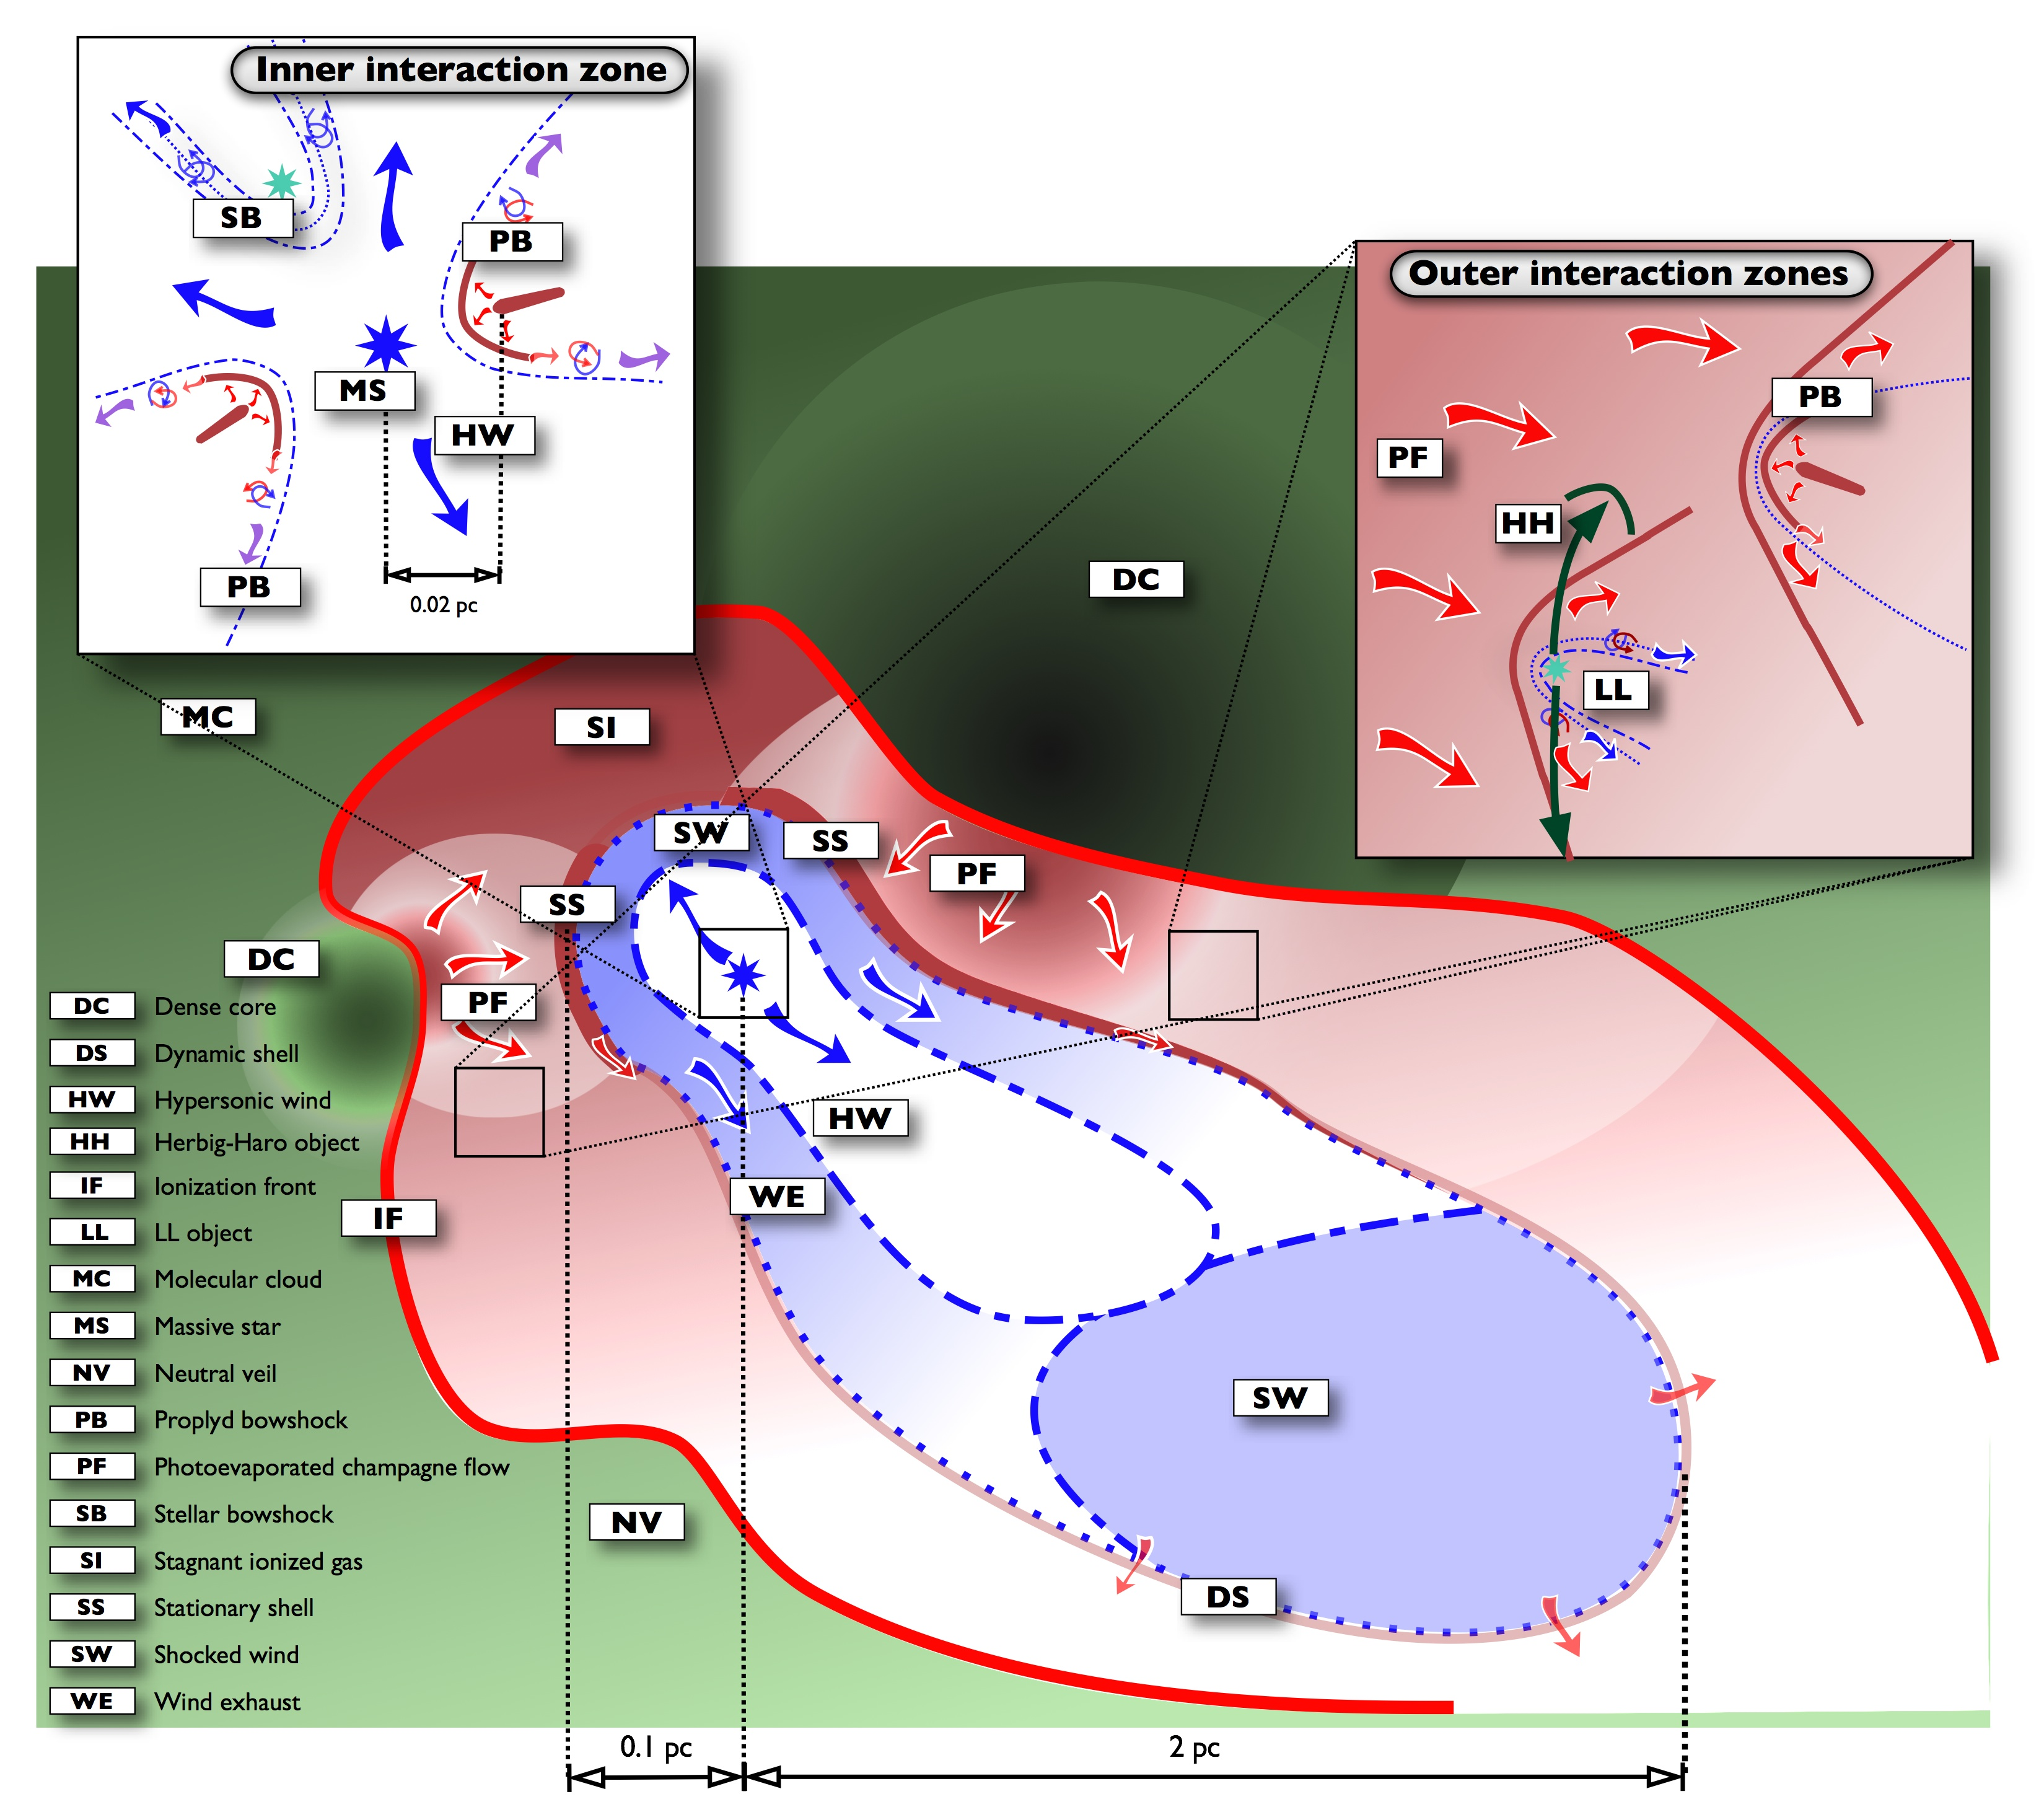
\includegraphics[width=\textwidth]{puebla-figs/wind-geometry-extended}
\end{frame}


\begin{frame}
  \frametitle{Two-shock stationary flow pattern}
  \centering\includegraphics[width=\textwidth]{balti-figs/LL-outer-inner}
\end{frame}

\subsection{Bowshock orientations}



\begin{frame}
  \frametitle{Orientation of the bowshocks in Orion}
  \centering
  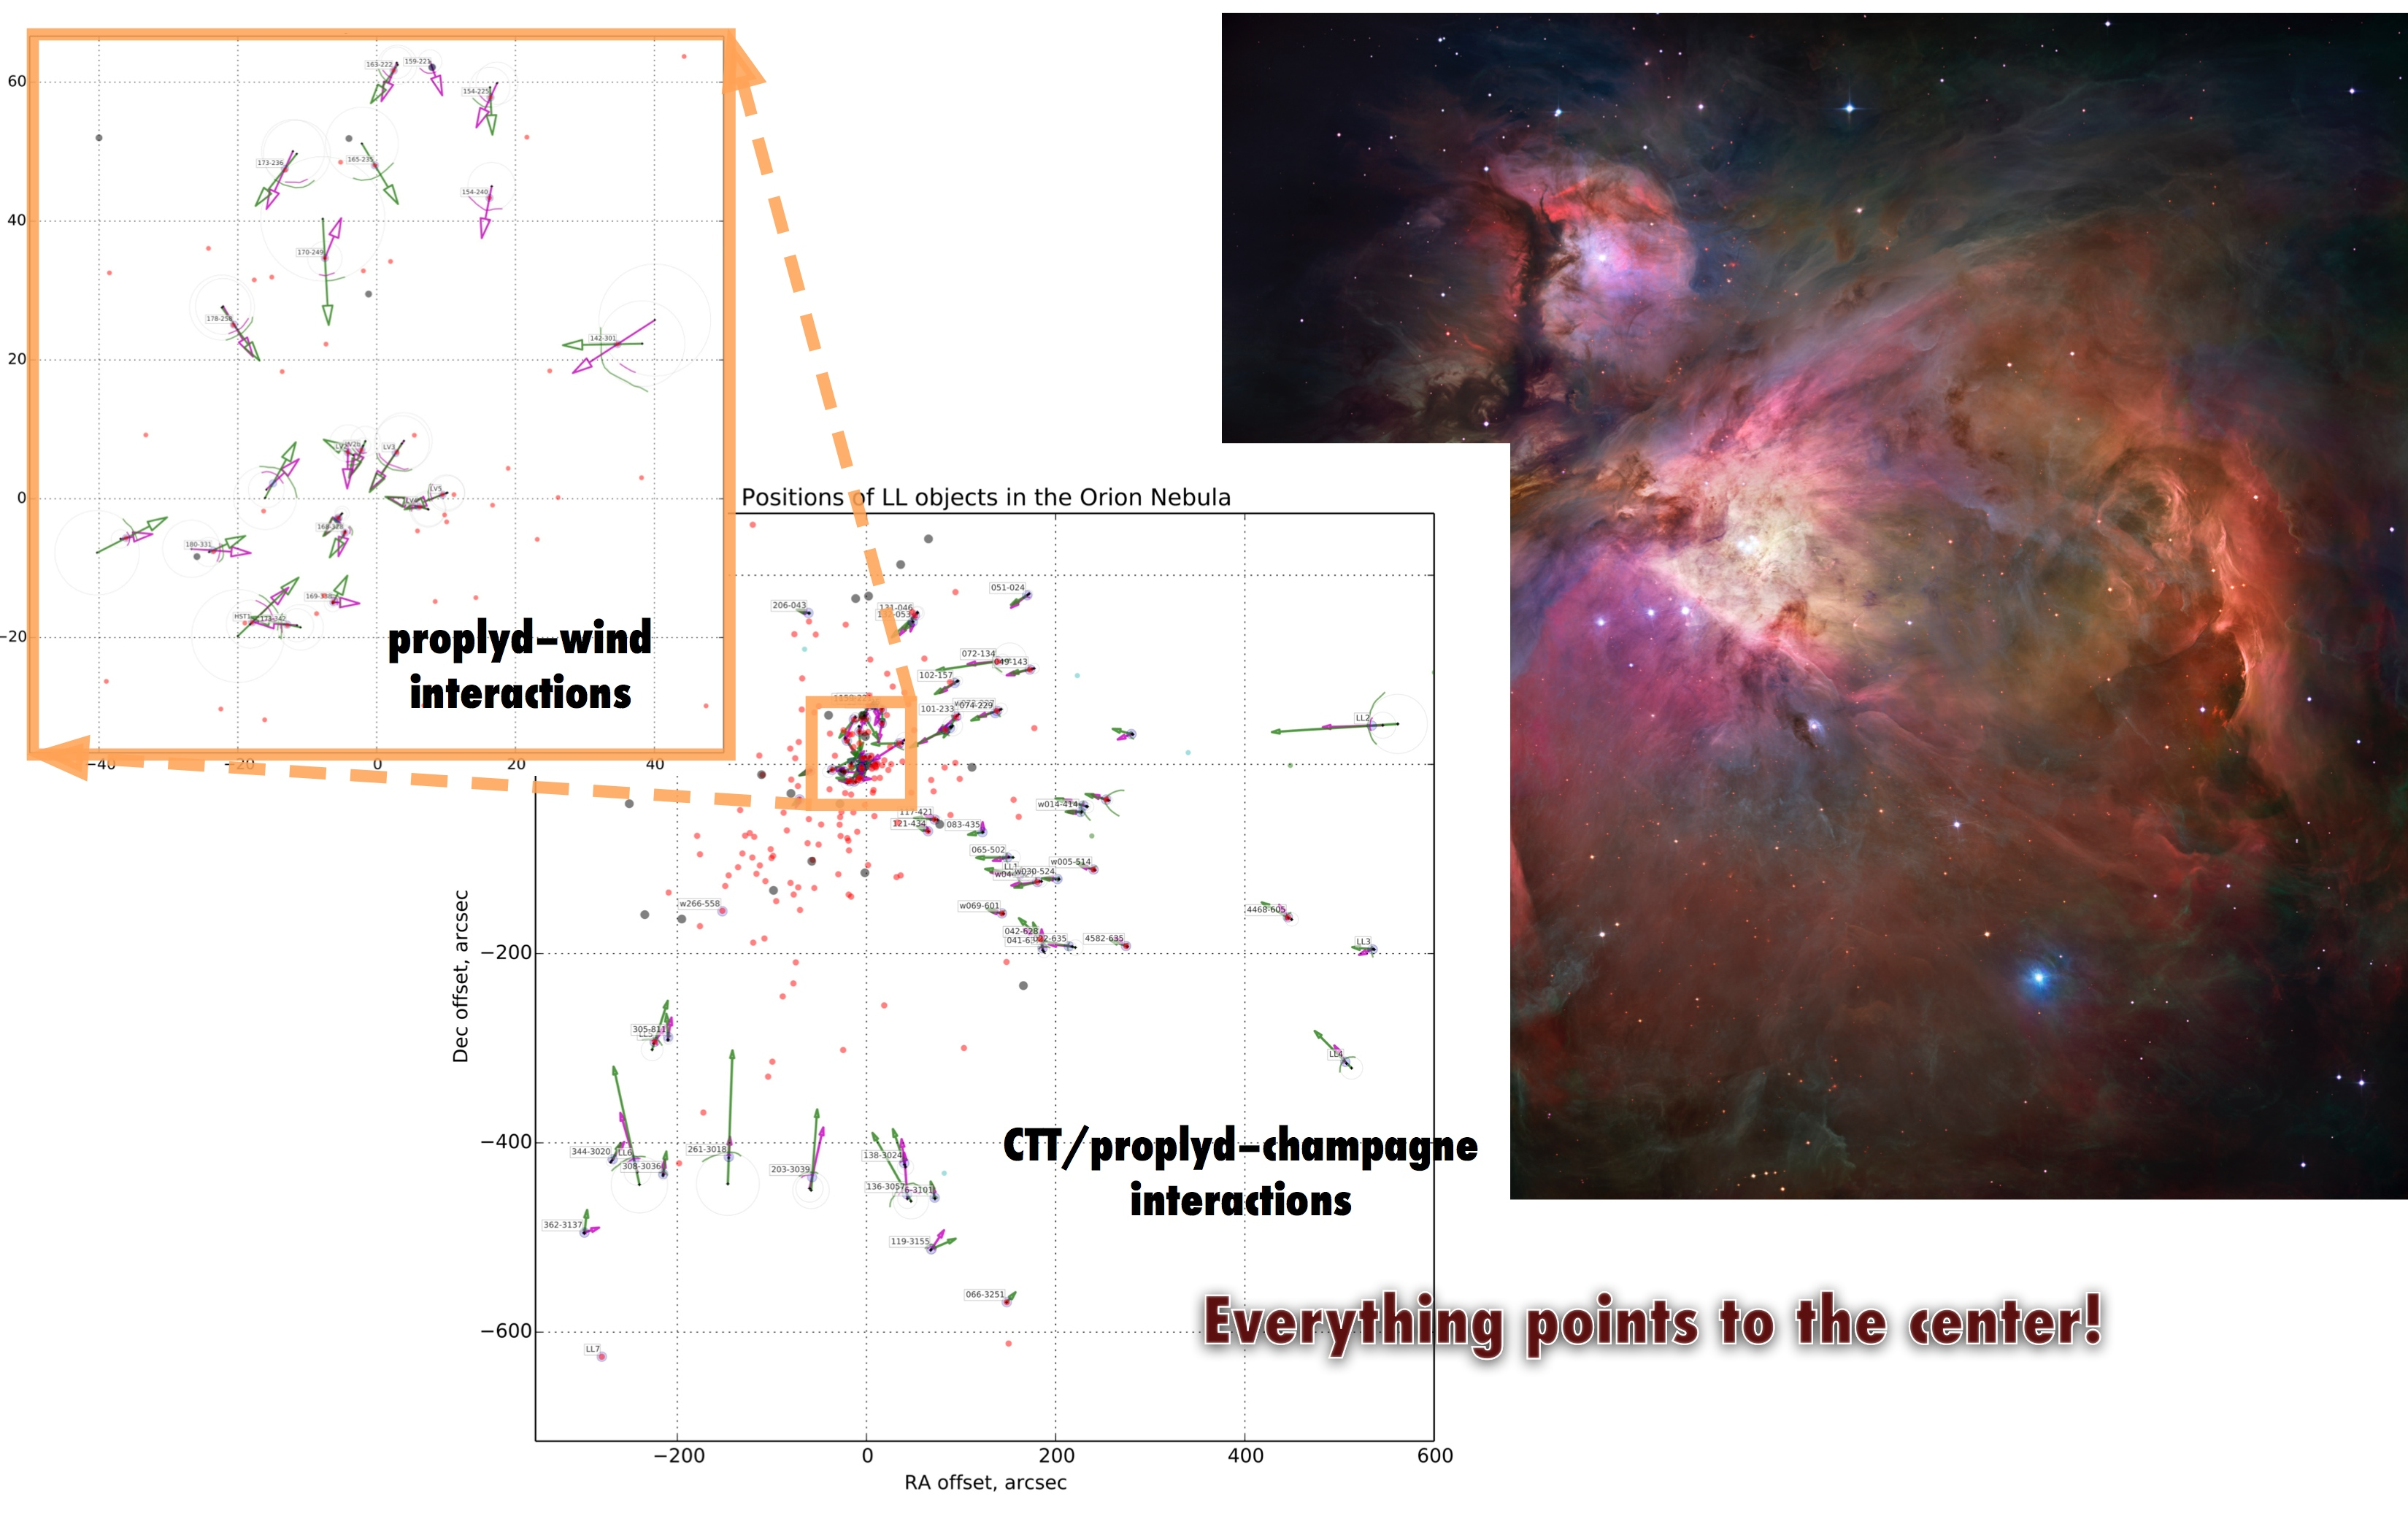
\includegraphics[width=\textwidth]{puebla-figs/LL-Positions-Combo}
\end{frame}

\subsection{Summary}

\begin{frame}
  \frametitle{Stellar winds: summary}
  
  \begin{enumerate}
  \item O-star winds are confined to the center of \hii{}
    regions
    \begin{itemize}
    \item They almost never dominate the appearance or dynamics
    \item (except maybe in low-density blow-outs)
    \end{itemize}
  \item Stellar bow shocks are not necessarily due to interactions
    with a hypersonic wind
    \begin{itemize}
    \item Transonic interactions with champagne/photoevaporation flows\\
      are more common
    \end{itemize}
  \item \textit{Please go and read the posters by Tarango et al.\ and
      Guti\'errez et al}.
  \end{enumerate}
  \bigskip
  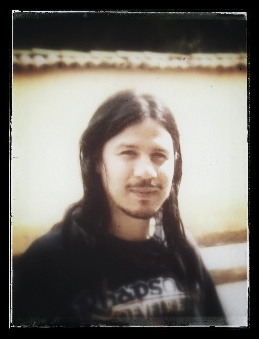
\includegraphics[height=0.3\textwidth]{puebla-figs/jorge-fancy}
  \includegraphics[height=0.3\textwidth]{poster-jorge-2014-small}
  
\includegraphics[height=0.3\textwidth]{puebla-figs/luis-fancy}
  \includegraphics[height=0.3\textwidth]{poster-luis-2014-small}
\end{frame}


\end{document}

\section{Effects of Stellar Winds}


\begin{frame}
  \frametitle{Slicing the velocity cubes}
  \foreach \y [count=\x] in {52,53,...,85} {%
    \only<\x>{\includegraphics[page=\y, trim=0 30 0 75,clip]{oldtalks/windsor-talk.pdf}}%
  }%
\end{frame}

\begin{frame}
  \frametitle{Global versus Local Champagne flows}
  Hello
\end{frame}



\end{document}
